\chapter{Plataforma de desarrollo}
\label{cap:capitulo3}

\begin{flushright}
\begin{minipage}[]{10cm}
\emph{Las herramientas adecuadas en las manos adecuadas pueden cambiar el mundo}\\
\end{minipage}\\

Steve Jobs\\
\end{flushright}

\vspace{1cm}

Tras haber establecido los objetivos que se pretenden alcanzar en este proyecto, en este capítulo se van a tratar las distintas plataformas de desarrollo tanto \textit{hardware} como \textit{software} que han contribuido para lograr dichos objetivos.

\section{Hardware}

(añadir esquema en fritzing completo)

\subsection{Raspberry pi}


\begin{figure} [h!]
	\begin{center}
		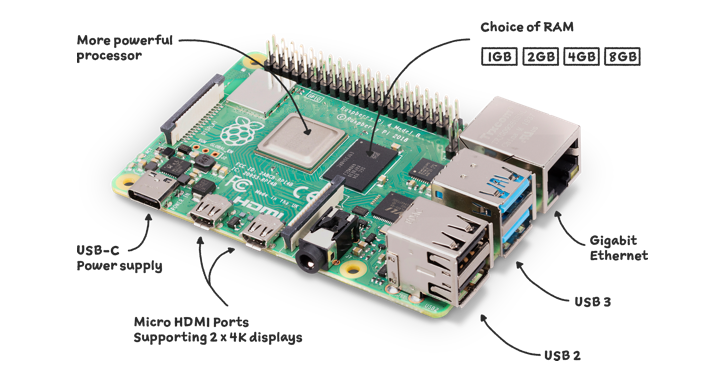
\includegraphics[width=8cm]{figs/raspberrypi4.png}
	\end{center}
	\caption{Raspberry Pi 4$^{\ref{note:enlace33}}$} 
\label{fig:raspberry}
\end{figure}\

\setcounter{footnote}{33} % Establecer la numeración de la siguiente nota al pie
\footnotetext[\value{footnote}]{\url{https://www.raspberrypi.com/products/raspberry-pi-4-model-b/}\label{note:enlace33}}


\subsection{Raspberry pi cámara}


\begin{figure} [h!]
	\begin{center}
		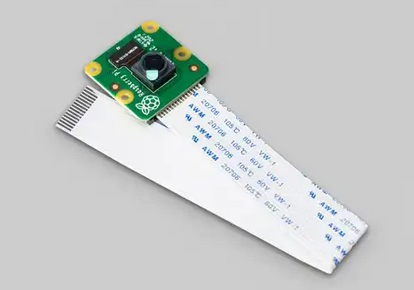
\includegraphics[width=6cm]{figs/campi.png}
	\end{center}
	\caption{Raspberry Pi Cámara V2$^{\ref{note:enlace34}}$} 
\label{fig:raspberrycam}
\end{figure}\

\setcounter{footnote}{34} % Establecer la numeración de la siguiente nota al pie
\footnotetext[\value{footnote}]{\url{https://www.raspberrypi.com/products/camera-module-v2/}\label{note:enlace34}}

\subsection{GPS NEO 6M}

\begin{figure} [h!]
	\begin{center}
		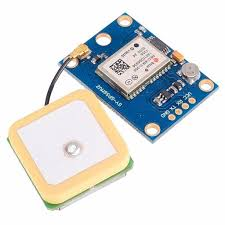
\includegraphics[width=4cm]{figs/GPSNEO6MV2.jpeg}
	\end{center}
	\caption{Módulo GPS NEO 6M$^{\ref{note:enlace35}}$} 
\label{fig:gps}
\end{figure}\

\setcounter{footnote}{35} % Establecer la numeración de la siguiente nota al pie
\footnotetext[\value{footnote}]{\url{https://www.amazon.es/dp/B088LR3488?ref=cm_sw_r_mwn_dp_4PA5Z4MX9MZZAKGSJ97G&ref_=cm_sw_r_mwn_dp_4PA5Z4MX9MZZAKGSJ97G&social_share=cm_sw_r_mwn_dp_4PA5Z4MX9MZZAKGSJ97G&language=en_US}\label{note:gps}}


\subsection{Sevomotores Parallax}

\begin{figure} [h!]
	\begin{center}
		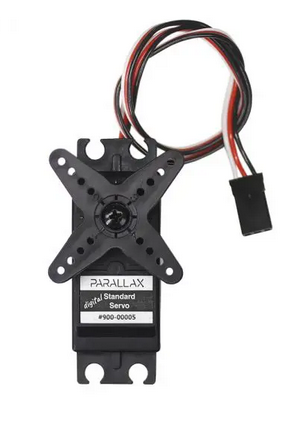
\includegraphics[width=4cm]{figs/parallax.png}
	\end{center}
	\caption{Servomotor Parallax$^{\ref{note:enlace36}}$} 
\label{fig:parallax}
\end{figure}\

\setcounter{footnote}{36} % Establecer la numeración de la siguiente nota al pie
\footnotetext[\value{footnote}]{\url{https://www.parallax.com/product/parallax-standard-servo/}\label{note:enlace36}}

\subsection{Ruedas ActivityBot}

\begin{figure} [h!]
	\begin{center}
		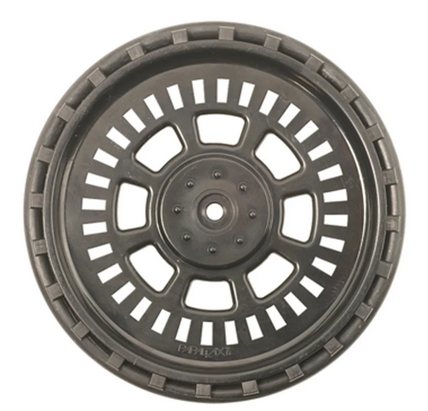
\includegraphics[width=4cm]{figs/wheel.png}
	\end{center}
	\caption{Rueda ActivityBot$^{\ref{note:enlace37}}$} 
\label{fig:wheel}
\end{figure}\

\setcounter{footnote}{37} % Establecer la numeración de la siguiente nota al pie
\footnotetext[\value{footnote}]{\url{https://es.rs-online.com/web/p/accesorios-para-kits-de-desarrollo/8430897?srsltid=AfmBOorv3a6_tQNdqAoKx_21Mn1m2MAum68oApyvr5mq8ExPTuh_CVNy}\label{note:enlace37}}

\subsection{Google Coral USB}

\begin{figure} [h!]
	\begin{center}
		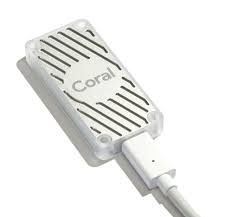
\includegraphics[width=4cm]{figs/googlecoral.png}
	\end{center}
	\caption{Google Coral USB$^{\ref{note:enlace38}}$} 
	\label{fig:googlecoral}
\end{figure}\

\setcounter{footnote}{38} % Establecer la numeración de la siguiente nota al pie
\footnotetext[\value{footnote}]{\url{https://coral.ai/products/accelerator/}\label{note:enlace38}}

\subsection{PowerBank}

\begin{figure} [h!]
	\begin{center}
		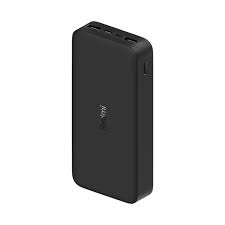
\includegraphics[width=4cm]{figs/powerbank.png}
	\end{center}
	\caption{Xiaomi Powerbank$^{\ref{note:enlace39}}$} 
	\label{fig:powerbank}
\end{figure}\

\setcounter{footnote}{39} % Establecer la numeración de la siguiente nota al pie
\footnotetext[\value{footnote}]{\url{https://buy.mi.com/es/item/3202200053}\label{note:enlace39}}

\subsection{Rueda Loca}


\begin{figure} [h!]
	\begin{center}
		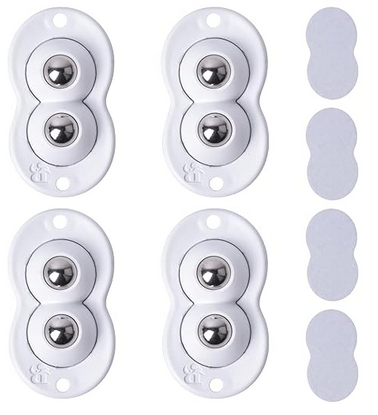
\includegraphics[width=4cm]{figs/ruedaloca.png}
	\end{center}
	\caption{Rueda loca$^{\ref{note:enlace40}}$} 
	\label{fig:ruedaloca}
\end{figure}\

\setcounter{footnote}{40} % Establecer la numeración de la siguiente nota al pie
\footnotetext[\value{footnote}]{\url{https://www.amazon.es/dp/B0BZZCJJT8?ref=cm_sw_r_mwn_dp_N64JV6SGENWN4YPSD849&ref_=cm_sw_r_mwn_dp_N64JV6SGENWN4YPSD849&social_share=cm_sw_r_mwn_dp_N64JV6SGENWN4YPSD849&language=es-ES}\label{note:enlace40}}

\subsection{Ordenador principal}


\begin{figure} [h!]
	\begin{center}
		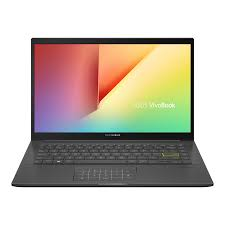
\includegraphics[width=4cm]{figs/ordenador.png}
	\end{center}
	\caption{ASUS VivoBook (añadir versión)$^{\ref{note:enlace41}}$} 
	\label{fig:ordenador}
\end{figure}\

\setcounter{footnote}{41} % Establecer la numeración de la siguiente nota al pie
\footnotetext[\value{footnote}]{\url{https://www.asus.com/es/laptops/for-home/vivobook/vivobook-14-k413/}\label{note:ordenador}}

\section{Software}

\subsection{Freecad}

\begin{figure} [h!]
	\begin{center}
		
\includegraphics[width=4cm]{figs/freecad.png}
	\end{center}
	\caption{Logo de Freecad $^{\ref{note:enlace42}}$} 
	\label{fig:freecad}
\end{figure}\

\setcounter{footnote}{42} % Establecer la numeración de la siguiente nota al pie
\footnotetext[\value{footnote}]{\url{https://www.freecad.org/}\label{note:enlace42}}

\subsection{Python}

\begin{figure} [h!]
	\begin{center}
		
\includegraphics[width=4cm]{figs/python.png}
	\end{center}
	\caption{Logo de Python $^{\ref{note:enlace43}}$} 
	\label{fig:python}
\end{figure}\

\setcounter{footnote}{43} % Establecer la numeración de la siguiente nota al pie
\footnotetext[\value{footnote}]{\url{https://es.python.org/}\label{note:enlace43}}

\subsection{OpenCV}

\begin{figure} [h!]
	\begin{center}
		
\includegraphics[width=4cm]{figs/opencv.png}
	\end{center}
	\caption{Logo de OpenCV $^{\ref{note:enlace44}}$} 
	\label{fig:opencv}
\end{figure}\

\setcounter{footnote}{44} % Establecer la numeración de la siguiente nota al pie
\footnotetext[\value{footnote}]{\url{https://opencv.org/}\label{note:enlace44}}

\subsection{Software matemático}

numpy

\subsection{Software localización}
pynmea

\subsection{Ubuntu}

\begin{figure} [h!]
	\begin{center}
		
\includegraphics[width=4cm]{figs/ubuntu.png}
	\end{center}
	\caption{Logo de Ubuntu $^{\ref{note:enlace45}}$} 
	\label{fig:ubuntu}
\end{figure}\

\setcounter{footnote}{45} % Establecer la numeración de la siguiente nota al pie
\footnotetext[\value{footnote}]{\url{https://ubuntu.com/}\label{note:enlace45}}

\subsubsection{Ubuntu 22.04}

\subsubsection{Ubuntu 20.04}


\subsection{ROS2}


\subsubsection{ROS2 Humble}

\subsubsection{ROS2 Foxy}


\begin{figure}[ht!]
	\centering
	\begin{minipage}{0.4\linewidth}
		\centering
		
\includegraphics[width=\linewidth]{figs/foxy.png}
		\caption*{\centering Ros2 Foxy $^{\ref{note:enlace46}}$} %\cite{memnon_image}
	\end{minipage}
	\hspace{2cm}
	% aquí incluir iamgen de Guerrero de terracota
	\begin{minipage}{0.35\linewidth}
		\centering
		
\includegraphics[width=\linewidth]{figs/humble.png}
		\caption*{\centering Logo Ros2 Humble $^{\ref{note:enlace47}}$} %\cite{gomezguerreros}
	\end{minipage}
	\caption{Distribuciones de ROS2 usadas}
	\label{fig:rosdis}
\end{figure}


% Definir la primera nota al pie con el número 1
\setcounter{footnote}{46} % Reiniciar la numeración de notas al pie
\footnotetext[\value{footnote}]{\url{https://docs.ros.org/en/foxy/Installation.html}\label{note:enlace46}}

\setcounter{footnote}{47} % Reiniciar la numeración de notas al pie
\footnotetext[\value{footnote}]{\url{https://docs.ros.org/en/humble/index.html}\label{note:enlace47}}


(condensar en herramientas de simulación?? añadir xml?? sdf...)
\subsection{Ros2 Control}

\subsection{Gazebo}


\begin{figure} [h!]
	\begin{center}
		
\includegraphics[width=4cm]{figs/gazebo.png}
	\end{center}
	\caption{Logo de Gazebo $^{\ref{note:enlace48}}$} 
	\label{fig:gazebo}
\end{figure}\

\setcounter{footnote}{48} % Establecer la numeración de la siguiente nota al pie
\footnotetext[\value{footnote}]{\url{https://gazebosim.org/home}\label{note:enlace48}}

\subsection{Herramientas de visualización}

rqtimage view

Rviz
ros2 topic echo...

\begin{figure} [h!]
	\begin{center}
		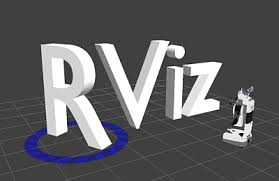
\includegraphics[width=4cm]{figs/rviz.png}
	\end{center}
	\caption{Logo de Rviz $^{\ref{note:enlace49}}$} 
	\label{fig:rviz}
\end{figure}\

\setcounter{footnote}{49} % Establecer la numeración de la siguiente nota al pie
\footnotetext[\value{footnote}]{\url{http://wiki.ros.org/rviz}\label{note:enlace49}}

\subsection{Google Colab/Jupyter Notebook}

\begin{figure} [h!]
	\begin{center}
		
\includegraphics[width=4cm]{figs/googlecolab.png}
	\end{center}
	\caption{Logo de Google Colab $^{\ref{note:enlace50}}$} 
	\label{fig:googlecolab}
\end{figure}\

\setcounter{footnote}{50} % Establecer la numeración de la siguiente nota al pie
\footnotetext[\value{footnote}]{\url{https://colab.research.google.com/}\label{note:enlace50}}

\subsection{YOLOv8}


\begin{figure} [h!]
	\begin{center}
		
\includegraphics[width=4cm]{figs/yolov8.png}
	\end{center}
	\caption{Logo de YOLOv8 $^{\ref{note:enlace51}}$} 
	\label{fig:yolov8}
\end{figure}\

\setcounter{footnote}{51} % Establecer la numeración de la siguiente nota al pie
\footnotetext[\value{footnote}]{\url{https://docs.ultralytics.com/es}\label{note:enlace51}}


\subsection{TensorFlow Lite Edge TPU}

\begin{figure} [h!]
	\begin{center}
		
\includegraphics[width=6cm]{figs/tflite.png}
	\end{center}
	\caption{Logo de TensorFlow Lite $^{\ref{note:enlace52}}$} 
	\label{fig:tflite}
\end{figure}\

\setcounter{footnote}{52} % Establecer la numeración de la siguiente nota al pie
\footnotetext[\value{footnote}]{\url{https://ai.google.dev/edge/litert}\label{note:enlace52}}


\subsection{Interfaz Web}

\subsubsection{ROS2 bridge suite}

\subsubsection{Open Street Maps}


\begin{figure} [h!]
	\begin{center}
		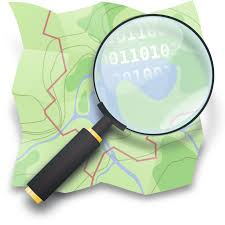
\includegraphics[width=4cm]{figs/osm.png}
	\end{center}
	\caption{Logo de Open Street Maps $^{\ref{note:enlace53}}$} 
	\label{fig:osm}
\end{figure}\

\setcounter{footnote}{53} % Establecer la numeración de la siguiente nota al pie
\footnotetext[\value{footnote}]{\url{https://www.openstreetmap.org}\label{note:enlace53}}


Mirar si hay que añadir alguna otra subsubsección
El presente proyecto trata ....\\


Después de aquí pasar al aparatado del estado del arte \\\\

En los textos puedes poner palabras en \textit{cursiva}, para aquellas expresiones en sentido \textit{figurado}, palabras como \textit{robota}, que está fuera del diccionario castellano, o bien para resaltar palabras de una colección: \textit{(a)} es la primera letra del abecedario, \textit{(b)} es la segunda, etc.\\

Al poner las dos líneas del anterior párrafo, este aparecerá separado del anterior. Si no las pongo, los párrafos aparecerán pegados. Sigue el criterio que consideres más oportuno.

\section{Segunda sección}
\label{sec:segundaseccion}

No olvides incluir imágenes y referenciarlas, como la Figura \ref{fig:roomba}.

\begin{figure} [h!]
	\begin{center}
		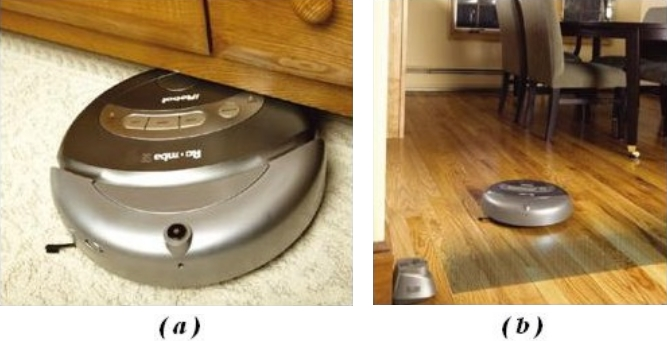
\includegraphics[width=8cm]{figs/roomba}
	\end{center}
	\caption{Robot aspirador Roomba de iRobot.}
	\label{fig:roomba}
\end{figure}\

Ni tampoco olvides de poner las URLs como notas al pie. Por ejemplo, si hablo de la Robocup\footnote{\url{http://www.robocup.org}}.

\subsection{Números}
\label{sec:subseccion}

En lugar de tener secciones interminables, como la Sección \ref{sec:robotica}, divídelas en subsecciones.

Para hablar de números, mételos en el entorno \textit{math} de \LaTeX, por ejemplo, $1.5Kg$. También puedes usar el símbolo del Euro como aquí: 1.500\euro.

\subsection{Listas}

Cuando describas una colección, usa \texttt{itemize} para ítems o \texttt{enumerate} para enumerados. Por ejemplo:

\begin{itemize}
	\item \textit{Entorno de simulación.} Hemos usado dos entornos de simulación: uno en 3D y otro en 2D.
	\item \textit{Entornos reales.} Dentro del campus, hemos realizado experimentos en Biblioteca y en el edificio de Gestión.
\end{itemize}\

\begin{enumerate}
	\item Primer elemento de la colección.
	\item Segundo elemento de la colección.
\end{enumerate}\

\paragraph{Referencias bibliográficas}
\label{sec:referencias}

Cita, sobre todo en este capítulo, referencias bibliográficas que respalden tu argumento. Para citarlas basta con poner la instrucción \verb|\cite| con el identificador de la cita. Por ejemplo: libros como \cite{vega12e}, artículos como \cite{vega19b}, URLs como \cite{vega19a}, tesis como \cite{vega18b}, congresos como \cite{vega18a}, u otros trabajos fin de grado como \cite{vega08b}.

Las referencias, con todo su contenido, están recogidas en el fichero \texttt{bibliografia.bib}. El contenido de estas referencias está en formato \texttt{BibTex}. Este formato se puede obtener en muchas ocasiones directamente, desde plataformas como \texttt{Google Scholar} u otros repositorios de recursos científicos.

Existen numerosos estilos para reflejar una referencia bibliográfica. El estilo establecido por defecto en este documento es APA, que es uno de los estilos más comunes, pero lo puedes modificar en el archivo \texttt{memoria.tex}; concretamente, cambiando el campo \verb|apalike| a otro en la instrucción \verb|\bibliographystyle{apalike}|. 

\

\

\

Y, para terminar este capítulo, resume brevemente qué vas a contar en los siguientes.
